\section{Xây dựng hệ cơ sở dữ liệu}\label{3.1}
Cơ sở dữ liệu cho thuật toán như hình ảnh dưới đây. 

\begin{figure}[H]
    \centering
    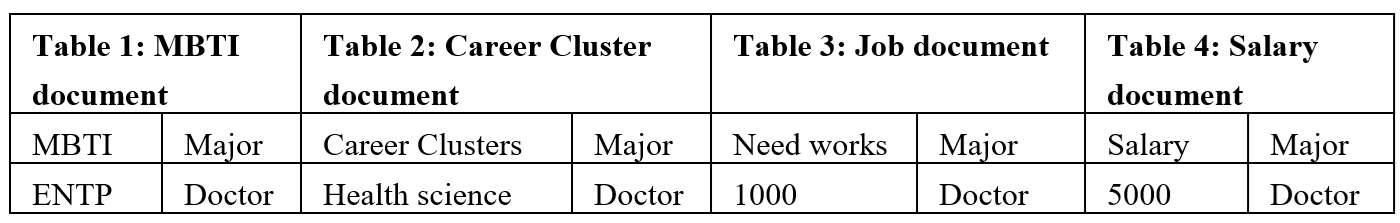
\includegraphics[width=0.8\linewidth]{images/chap3/data.png}
    \vspace{0.5cm}
    \caption{Hình ảnh cơ sở dữ liệu cho thuật toán}
\end{figure}

Đối với dữ liệu về MBTI và ngành nghề, dữ liệu được lấy từ cuốn sách ``\textit{Chọn nghề theo tính cách}" của Alpha Book \cite{alpha}. Cuốn sách ``\textit{Chọn Nghề Theo Tính Cách}” của Alpha Books là một cuốn sách rất gần gũi và dễ đọc, vừa theo dạng câu chuyện vừa theo dạng một cẩm nang hướng dẫn. Sách được chia thành hai phần chính, trong đó đặc biệt là phần 2. Hướng dẫn chọn nghề: Phần này hướng dẫn bạn cách tìm ra nghề nghiệp yêu thích và phù hợp với bản thân. Mục tiêu của cuốn sách là cung cấp cho bạn cách thức chọn nghề hữu hiệu nhằm giúp bạn tìm được nghề nghiệp phù hợp nhất với bản thân mình. Để đạt được mục tiêu này, người đọc sẽ cần đọc hiểu một số phần và bỏ ra chút công sức suy nghĩ và hoàn thành những phần khác. Cảm ơn cuốn sách đã góp phần xây dựng hệ cơ sở dữ liệu cho chúng tôi. 

Bên cạnh đó, nhóm cũng tham khảo dựa vào loạt bài viết về MBTI trên trang web chính thức của trung tâm nghề nghiệp trường đại học Ball State, Ball State University Lucina Hall Room 220 Muncie, IN 47306. Nhóm đã dựa vào dữ liệu từ trang web này và cuốn sách ``Chọn nghề theo tính cách” để xây dựng dữ liệu về MBTI và ngành nghề, cũng như để trả lời cho câu hỏi ``\textit{what do you love?}” - điều gì bạn yêu thích. 

Đối với dữ liệu về Career Clustering và nghề nghiệp, nhóm xây dựng dựa trên dữ liệu về các nghề phân theo nhóm ngành dựa trên 16 cụm trong Career Clustering được công bố chính thức từ phòng công nghệ và giáo dục của Oklahoma, Mỹ (thông tin chi tiết có thể xem tại website chính thức được công bố). Hình 3.3 thể hiện thông tin về phòng công nghệ và giáo dục Oklahoma, Mỹ.

\begin{figure}[H]
    \centering
    
\includegraphics[width=0.65\linewidth]{images/chap3/oklahomaInfo.png}
    \vspace{0.5cm}
    \caption{Thông tin về Phòng Công nghệ và Giáo dục Oklahoma, Mỹ}
\end{figure}

Đối với dữ liệu về tiền lương và các ngành nghề, cũng là để trả lời cho câu hỏi ``Điều gì đem lại thu nhập cho bạn" (\textit{What will pay for you?}). Nhóm sử dụng dữ liệu được công bố chính thức của bộ phận thống kê của tổ chức lao động thế giới - ILOSTAT về \textit{Average monthly earning by sex and occupation} - Thu nhập hằng tháng theo giới tính và độ tuổi. Bên cạnh đó, nhóm cũng sử dụng dữ liệu từ Vietnam Salary của CareerViet. Vietnam Salary của CareerViet là một dịch vụ khảo sát mức lương và là một mạng lưới việc làm và tuyển dụng hàng đầu thế giới với hơn 2 triệu việc làm và hơn 200 triệu ứng viên trên 72 quốc gia toàn cầu. Vietnam Salary cung cấp thông tin về mức lương tại Việt Nam, giúp người dùng có cái nhìn tổng quan về mức lương hiện hành tại thị trường. Điều này rất hữu ích cho cả nhà tuyển dụng và người tìm việc, giúp họ đưa ra quyết định tốt nhất dựa trên thông tin mức lương. Ngoài ra, với những ngành nghề đặc thù, nhóm sử dụng dữ liệu được quy định trong các văn bản hành chính mới nhất như văn bảng quy định mức lương chính thức của công chức nhà nước hay ngành công an \cite{thuvienphapluat} \cite{tuoitre} \cite{hocmai} \cite{umt} \cite{topcv} \cite{xaydungchinhsach}.

\begin{figure}[H]
    \centering
    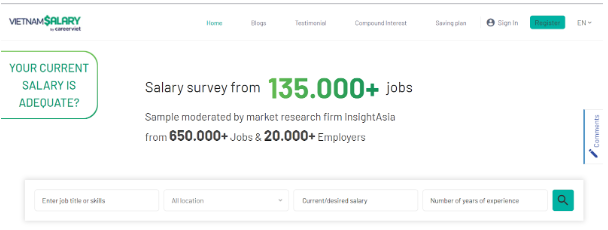
\includegraphics[width=0.8\linewidth]{images/chap3/VietnamSalary.png}
    \vspace{0.6cm}
    \caption{Trang web VietnamSalary}
\end{figure}

Đối với dữ liệu về ngành nghề và việc làm, nhóm xây dựng dựa trên dữ liệu của Tổng cục thống kê, thuộc Bộ Kế Hoạch và Đầu Tư của Việt Nam, về số lao động có việc làm và cơ cấu lao động có việc làm trong nền kinh tế phân theo ngành kinh tế. Ngoài ra, nhóm còn sử dụng dữ liệu trực tuyến được cung cấp bởi LinkedIn. LinkedIn là một mạng xã hội chuyên nghiệp hàng đầu thế giới, cung cấp một nền tảng cho người dùng để kết nối với nhau và tìm kiếm cơ hội nghề nghiệp, cho cả những ngành đặc thù như công nhân viên chức, công an, giáo viên. Nhóm sử dụng số liệu chính thức được các trang web của các bộ, ban ngành cung cấp để xây dựng cơ sở dữ liệu \cite{xaydungdang} \cite{vietnamnet} \cite{cafef}.

Đối với dữ liệu về ngành học và việc làm, nhóm sử dụng dữ liệu được thu thập từ trang web chính thức tử các trường đại học hàng đầu tại Việt Nam như đại học Bách Khoa, đại học Ngoại Thương, đại học Kinh Tế Thành Phố Hồ Chí Minh để xây dựng, phân bố các ngành, cũng dựa vào dữ liệu gợi ý từ các chuyên gia hướng nghiệp, các tin tức chính thống đầu ngành để xây dựng, các hội thảo liên quan tới giáo dục, lựa chọn ngành nghề để xác định và trích dẫn thông tin như hội thảo ngành học của đại học RMIT 2023, Hội thảo về khoa học giáo dục 2023, hay các ngày tư vấn tuyển sinh và đặc biệt là chương trình BKFC của \acrlong{dhbk}.

Từ những điều đã nói ở trên, nhóm thông qua quá trình trích chọn, cân nhắc, xây dựng hệ cơ sở dữ liệu đối với mô hình hệ hỗ trợ quyết định dựa trên Ikigai. Dù vẫn còn nhiều thiếu sót nhưng nhóm xin gửi lời cảm ơn sâu sắc tới các cơ quan tổ chức đã cung cấp những nguồn dữ liệu mở, chính xác để nhóm có thể tiến hành xây dựng, phát triển đồ án này.